\chapter{Abstracte syntax}
\label{ch:abstract_syntax}
Abstract syntax tree stelt eerder semantiek voor, parse trees de constructieregels. De abstract syntax tree wordt opgebouwd tijdens het parsen.
\section{Semantische acties}


Een parser voert syntactische acties uit zoals shift en reduce. Een semantische actie heeft betrekking tot de betekenis van de expressies. Een aantal voorbeelden van het bepalen van semantische waarden:
\begin{itemize}
	\item Het type van het linkerlid bepalen van de expressie $a = 5 + 3$.
	\item Terminals en niet-terminals hebben semantische waarden van een bepaald type.
\end{itemize}

In een recursive-descent parser zijn de semantische acties de returnwaarden van de parsingfunctie. Voor elke terminaal en niet-terminaal symbool, wordt er een \textbf{type} geassocieerd van semantische waarden. Een eenvoudige rekenmachine wordt kan op deze manier \textit{geïnterpreteerd} worden, uitgewerkt op grammatica \ref{grammar_3_15} in code \ref{code:recursive_descent_parser_grammar315}.
\begin{grammarfigure}
	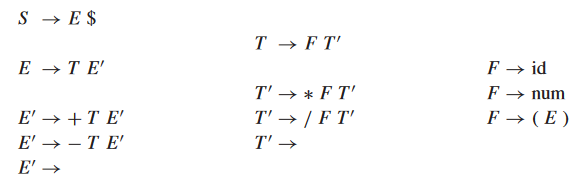
\includegraphics[width=\textwidth]{grammar_3_15}
	\caption{}
	\label{grammar_3_15}
\end{grammarfigure}


\begin{lstlisting}[caption={Recursive-descent parser voor grammatica \ref{grammar_3_15}.},label={code:recursive_descent_parser_grammar315},captionpos=b]
enum token {EOF, ID, NUM, PLUS, MINUS, ...};
union tokenval {string id; int num; ...};

enum token tok;
union tokenval tokval;

int lookup(string id) { ... }

void eatOrSkipTo(int expected, int* stop){
  if (tok == expected) eat (expected);
  else {printf(...); skipto(stop)}
}

int F_follow[] = { PLUS, TIMES, RPAREN, EOF, -1 };
int F(void) {switch (tok) {
  case ID:     {int i = lookup(tokval.id); advance(); return i;}
  case NUM:    {int i = tokval.num; advance(); return u;}
  case LPAREN: eat(LPAREN); int i = E(); eatOrSkipTo(RPAREN, F_follow); 
               return i; }
  case EOF:
  default:     printf("expected ID, NUM, or left-paren");
               skipto(F_follow);
               return 0;
  }}

int T_follow[] = { PLUS, RPAREN, EOF, - 1 };
int T(void) {switch (tok) {
  case ID: case NUM: case LPAREN: return Tprime(F());
  default: printf("expected ID, NUM, or left-paren");
           skipto(T_follow);
           return 0;
 }}
 
int Tprime(int a) {switch (tok) {
  case TIMES: eat(TIMES); return Tprime(a*F());
  case PLUS: case RPAREN: case EOF: return a;
  default: ...
  }}
\end{lstlisting}

De tokens \texttt{ID} en \texttt{NUM} moeten respectievelijk waarden van type \texttt{string} en \texttt{int} bevatten. De functie lookup kan een waarde zoeken voor een identifier. Zowel \texttt{E}, \texttt{T} als \texttt{F} is van type int.

In plaats van dit handmatig te doen, kan een tool gebruikt worden die dit genereerd zoals Yacc (look ahead left-to-right parser generator), zoals te zien in code \ref{code:yacc}.
\begin{lstlisting}[caption={Yacc.},captionpos=b,label={code:yacc}]
%{ declarations of yylex  and yyerror %}
%union {int num; string id;}
%token <num> INT
%token <id> ID
%type <num> exp
%start exp

%left PLUS MINUS
%left TIMES
%left UMINUS
%%

exp : INT            {$$ = $1;}
    | exp PLUS exp   {$$ = $1 + $3;}
    | exp MINUS exp  {$$ = $1 - $3;}
    | exp TIMES exp  {$$ = $1 * $3;}
    | MINUS exp      %prec UMINUS {$$ = - $2;}
\end{lstlisting}
Figuur \ref{fig:semantische_stack} toont een LR parse of een string, gebruik makend van code \ref{code:yacc}.
\begin{figure}[h]
	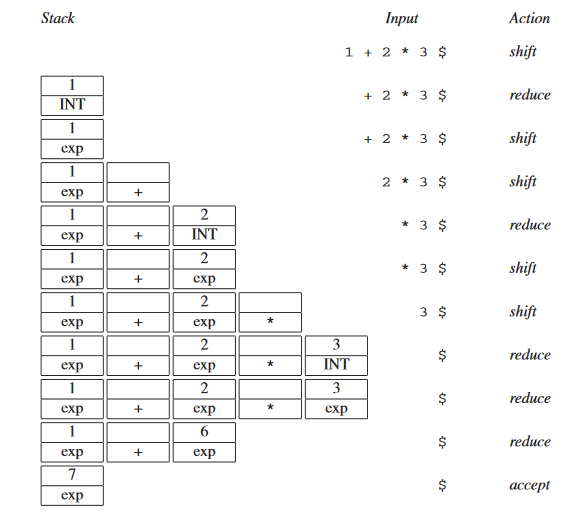
\includegraphics[width=\textwidth]{semantische_stack}
	\caption{Parsen met een semantische stack.}
	\label{fig:semantische_stack}
\end{figure}

Interpreteren met behulp van semantische acties is dus zeer haalbaar. In feite kan compilatie ook uitgevoerd worden met semantische acties, maar wordt in de praktijk afgeraden:
\begin{itemize}
	\item Analyse kan enkel uitgevoerd worden in de volgorde waarin de inputstream geparsed wordt. 
	\item Code wordt gegenereerd op basis van de parse tree, maar zo een tree is niet geschikt. Er zit te veel nutteloze informatie in zoals de := operator, en dient eerder om de syntax uit te drukken en niet de semantiek.
\end{itemize}

\section{Abstract Parse Tree Construction}
\begin{grammarfigure}[h]
	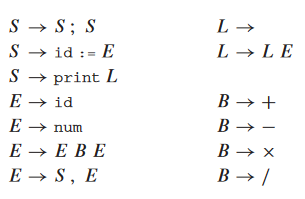
\includegraphics[width=\textwidth]{grammar_4_5}
	\caption{}
	\label{fig:grammar_4_5}
\end{grammarfigure}
In principe 
Grammatica 4.5 is ambigue. Binaire operator specificeert geen associativiteit. Dit is geen probleem, aangezien de parser dit al beslist heeft. Dus de grammatica die de parser gebruikt mag niet ambigue zijn, wel die van de abstract syntax tree, aangezien die dient om de semantiek te definiëren.
\subsection{Posities}
Als je tree opbouwt, wordt deze geanalyseerd om bv types te checken. Bij foutboodschappen moet de compiler weten waar in de inputstroom deze fout gegenereerd wordt. Er kan een \textbf{positiestack} bijgehouden worden die de positie van elke token bevat.